\usetikzlibrary{arrows.meta}
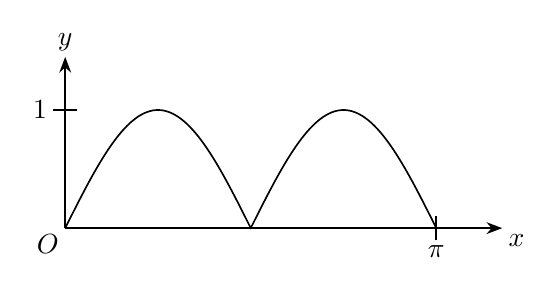
\begin{tikzpicture}[x=1.5cm,y=1.5cm,line width=.6pt,>=Stealth]
\draw[->] (0,0)--(3.7,0) node[below right,inner sep=2pt] {$x$};
\draw[->] (0,0)--(0,1.45) node[above,inner sep=2pt] {$y$};
\draw plot[domain=0:3.14159265,samples=241] (\x,{abs(sin(deg(2*\x)))});
\draw (-0.1,1)--(0.1,1);
\node[left,inner sep=2pt] at (-0.1,1) {$1$};
\draw (3.1416,-0.1)--(3.1416,0.1);
\node[below=5pt,inner sep=1pt] at (3.1416,0) {$\pi$};
\node[below left,inner sep=2pt] at (0,0) {$O$};
\end{tikzpicture}
